% This is a basic Math Paper

\documentclass[11pt]{article}

% Preamble

\usepackage[margin=1in]{geometry}
\usepackage{amsfonts, amsmath, amssymb}
\usepackage{fancyhdr, float, graphicx}
\usepackage[utf8]{inputenc} % Required for inputting international characters
\usepackage[T1]{fontenc} % Output font encoding for international characters
\usepackage{fouriernc} % Use the New Century Schoolbook font
\usepackage[nottoc, notlot, notlof]{tocbibind}
\usepackage{url}
\usepackage{placeins}
\usepackage{multirow}
% Header and Footer
\pagestyle{fancy}
\fancyhead{}
\fancyfoot{}
\fancyhead[L]{\textit{\Large{Experiment 4. Beam Divergence}}}
\fancyhead[R]{\textit{something}}
\fancyfoot[C]{\thepage}
\renewcommand{\footrulewidth}{1pt}



% Other Doc Editing
\parindent 0ex
\renewcommand{\baselinestretch}{1.3}

\begin{document}
	
	\begin{titlepage} 
		\centering 
		
		%---------------------------NAMES-------------------------------
		
		\huge\textsc{
			MIT World Peace University
		}\\
	
		\vspace{0.75\baselineskip} % space after Uni Name
		
		\LARGE{
			Physics\\
			First Year B. Tech, Trimester 3\\
			Academic Year 2021-22
		}
		
		\vfill % space after Sub Name
		
		%--------------------------TITLE-------------------------------
		
		\rule{\textwidth}{1.6pt}\vspace*{-\baselineskip}\vspace*{2pt}
		\rule{\textwidth}{0.6pt}
		\vspace{0.75\baselineskip} % Whitespace above the title
		
		
		
		\huge{\textsc{
				Measurement of Beam Divergence of a Laser Beam
			}} \\
		
		
		
		\vspace{0.5\baselineskip} % Whitespace below the title
		\rule{\textwidth}{0.6pt}\vspace*{-\baselineskip}\vspace*{2.8pt}
		\rule{\textwidth}{1.6pt}
		
		\vspace{1\baselineskip} % Whitespace after the title block

		%--------------------------SUBTITLE --------------------------	
			
		\LARGE\textsc{
			Experiment No. 4
		} % Subtitle or further description
		\vfill
		
		%--------------------------AUTHOR-------------------------------
		
		Prepared By
		\vspace{0.5\baselineskip} % Whitespace before the editors
		
		\Large{
			109054. Krishnaraj Thadesar
			
			Division 9 Batch I3
		}
		
		
		\vspace{0.5\baselineskip} % Whitespace below the editor list
		\today

	\end{titlepage}

	\begin{center}
	{\Large Pledge}\\
	\vspace{0.5cm}
	I solemnly affirm that I am presenting this journal based on my own experimental work. I have neither copied the observations, calculations, graphs and results from others nor given it to others for copying.\\
		\end{center}
	
	\vspace{0.5cm}
	
    \begin{flushright}
	{\large Signature of the student}\\
	\vspace{1cm}
	 \end{flushright}
	
	\section{Aim}
	\noindent
	To measure the peak power and beam divergence of a given laser beam

	
	\section{Apparatus}


		\begin{enumerate}
			\item He-Ne Laser
			\item Optical Bench
			\item Laser Beam Analyzer with Sensor
			\item Micrometer Screw Arrangement
		\end{enumerate}


	\section{Significance of the Experiment}
	\textit{One of the characteristics of laser is high
	directionality/parallelness. Thus the diameter of the laser at any position should be same.
	However, laser has a small divergence due to diffraction effects. This experiment provides an	
	easy and accurate method to measure the divergence of a laser}
	
	
	\section{Theory}

	\subsection{Lasers}
	Laser is an extremely coherent, monochromatic, directional, focusable, polarized and
powerful light. These extraordinary features make it greatly applicable in day-to-day life, science
and technology. A few notable applications of laser include medical diagnosis and treatments,
fiber optic communications, CD-ROMS, CD players, laser printers, defense, cutting, welding,
drilling, surveying, aligning etc.
Laser is produced due to stimulated radiation; a process where a resonating photon
stimulates the de-excitation of an excited atom. This results in to emission of two coherent
photons, which are identical in all respects. These photons further stimulate the de-excitation of
other excited atoms and this continues to generate an avalanche of coherent photons. For
stimulated emission to take over spontaneous emission and stimulated absorption, a few
conditions are necessary. These are availability of metastable state (life time = 10-3 sec),
population inversion (greater number of atoms in metastable state than in lower energy state) and
enough number of photons in the cavity (mirrors).

\subsection{He-Ne Lasers}

He-Ne laser is a low power, continuous gas laser, which is used in supermarket scanners, student
laboratories and holography. The active system is neon, which is pumped electronically via
helium in a resonant cavity made of discharge tube (Fig. 5.1) . The main lasing occurs in neon
between the levels E6 (metastable) and E3 which produces an intense coherent beam of red color
(wavelength 6328o). (refer Fig 5.2). The population of photons necessary for stimulated emission
is maintained by mirrors (one is semitransparent) on both sides. Brewseter windows are used to
polarize the laser light.

	\begin{figure}[H]
		\centering
		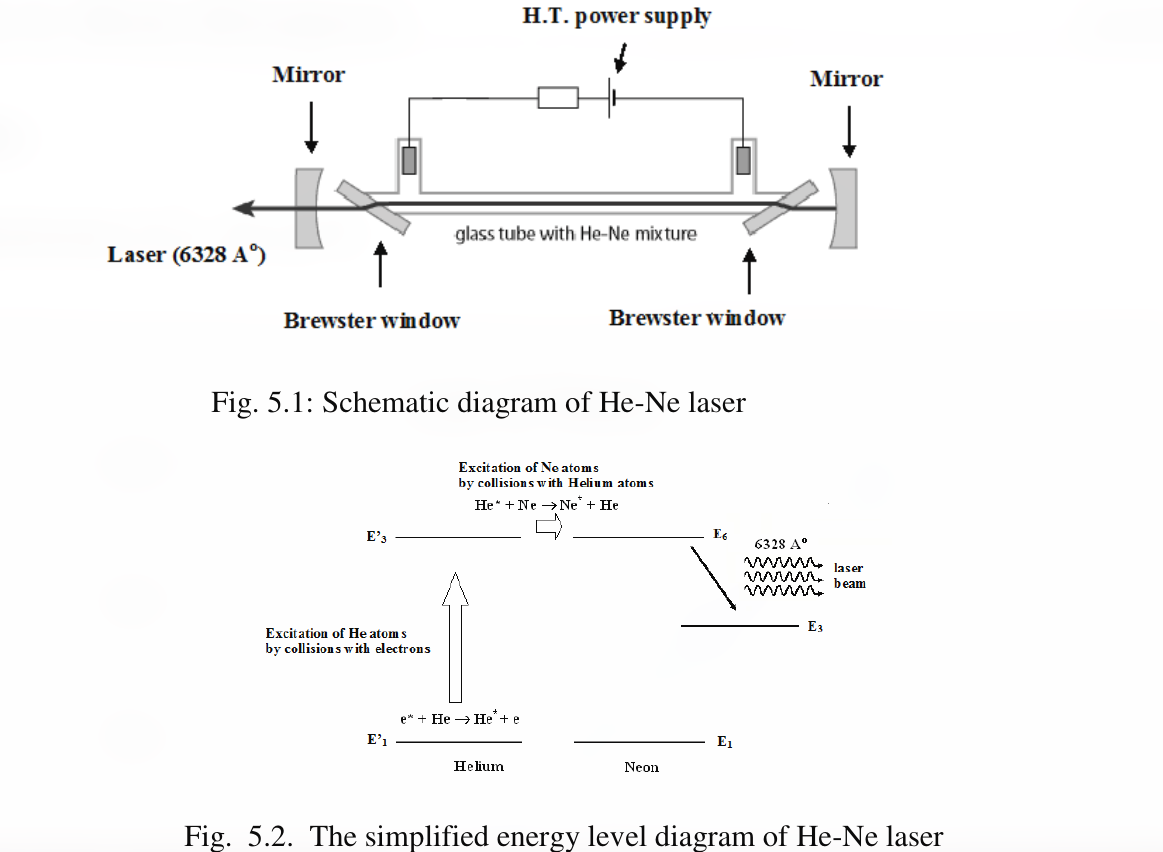
\includegraphics[scale=0.4]{1.png}
		\label{it}
	\end{figure}
	
\section{Procedure}
	
	\begin{enumerate}
	
	\item The power in laser beam follows Gaussian distribution with peak value at center.
 
	\item Mount the sensor of LBA on optical bench at a distance relatively closer to laser beam,
 say 10 cm. Let this distance be  $d_1$ . Adjust sensor so that laser is incident exactly on the
 centre of the window of the sensor. Align the sensor, till LBA reads power closest to 2.0
 mW
 \item Now move the sensor laterally so that the beam falls on the edge of the window of the
 sensor. LBA will now read zero.

 \item Using micrometer screw, move the sensor-window gradually across the laser beam. Note
 the increasing powers in the beam (mW) at various screw positions (mm) as per table 5.1. At certain stage, the power in LBA will reach peak and then will start decreasing,
 even though the screw is moved in the same direction. Note the decreasing powers at
 various advanced screw positions. Note that the screw should be moved in only one
 direction throughout the observations. For measuring the screw positions, use following
 procedure

	\begin{equation}
		\textit{Screw position} = X = MSR + VSR \times LC \textit{ mm}
	\end{equation}

	Where MSR is the reading on the main scale, which is
closest to the edge of the screw. VSR is the vernier scale
reading, which is the sequence number of the division on
the screw which coincides with the line on main scale.
LC is the least count of micrometer screw gauge

\begin{equation}
	LC = \frac{\textit{Smallest distance on the main scale}}{\textit{Number of divisions on the vernier scale}} = \frac{\dots mm}{\dots} = \dots mm
\end{equation}


\item Repeat the entire procedure from 2 to 4, by placing the sensor at  $d_2$ cm, sufficiently away
from  $d_1$(say by 50 cm). Record these observations in table 5.2


\item Plot the graph of power (mW) Vs position (mm) for observation table 5.1 (for \(d_1\)).
Identify the peak power \(P_m\). Also identify a point on power axis corresponding to \(P_m/2\).
Draw a horizontal line starting from \(\frac{P_m}{2}\).. This line will intersect the Gaussian curve at
two points having X co-ordinates $X_1$ (mm) and $X_2$ (mm). The quantity $D_1$ (mm) = $(X_2 - X_1)$
i.e. Full Width at Half Maximum (FWHM) gives the effective diameter of laser when the
distance between LBA and laser is $d_1$ cm. (refer sample graph in Fig. 5.3 a)

\item Plot the graph of power (mW) Vs position (mm) for observation table 2 (for  $d_2$). Repeat
the procedure explained in step 6 and calculate the diameter  $D_2$ (mm) of the laser beam at
the position  $d_2$. (refer a widened graph in Fig 5.3b)

\item The Gaussian distribution at the position $d_2$ will be slightly wider than that at position d1 .
Consequently the diameter  $D_2$ of the laser beam at the position $d_2$ will be greater than
diameter $D_1$ at the distance $d_1$. Calculate the divergence of laser beam by using the
formula and procedure in 'Calculations'

	\end{enumerate}
\clearpage

\section{Observations}

Table (3.1): Observations, Calculations and Results.

\begin{figure}[H]
	\centering
	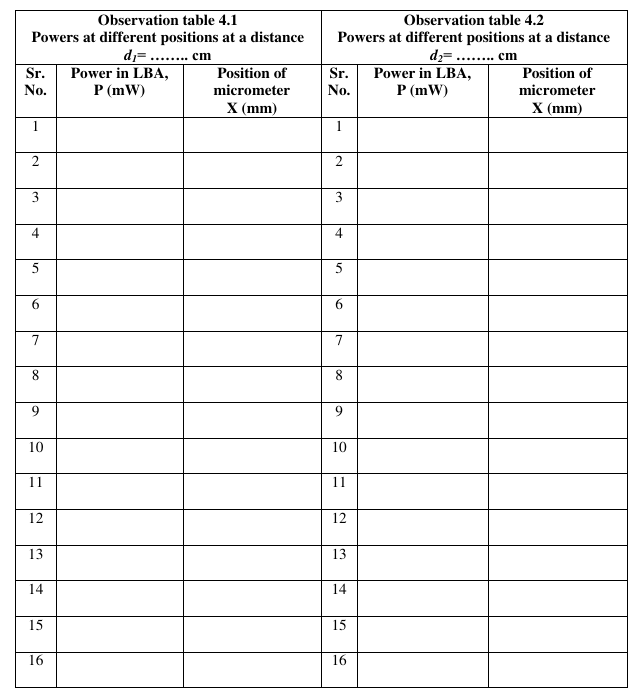
\includegraphics[scale=0.9]{table.png}
	\label{it}
\end{figure}

	\section{Calculations}

	$$
	\begin{aligned}
	\text { Divergence }=\frac{\left(D_{2}-D_{1}\right) \mathrm{mm}}{\left(d_{2}-d_{1}\right) \mathrm{cm}} \\
	=& \frac{\left(D_{2}-D_{1}\right) \mathrm{cm}}{\left(d_{2}-d_{1}\right) \mathrm{cm}} \times 10^{-1} \\
	=& \frac{(\ldots \ldots \ldots-\ldots \ldots)}{(\ldots \ldots \ldots-\cdots \ldots \ldots)} \times 10^{-1} \\
	=& \dots \ldots \ldots \ldots \mathrm{rad} \\
	=& \dots \ldots \ldots \ldots \ldots \mathrm{rad} \times \frac{180}{3.14} \frac{\mathrm{deg}}{\mathrm{rad}} \\
	=& \dots \ldots \ldots \ldots . \mathrm{deg} \\
	=& \dots \ldots \ldots \ldots \ldots \mathrm{deg} \times 60 \frac{\mathrm{min}}{\mathrm{deg}} \\
	=& \dots \ldots \mathrm{min}
	\end{aligned}
	$$

	\section{Results}
	\begin{centering}
	\begin{tabular}{|c|l|c|c|}
	\hline Sr. No. & \multicolumn{1}{|c|}{ Physical quantity } & Value & Unit \\
	\hline 1 & Peak power the laser beam $\left(\right.$ at $\left.d_{1} \ldots \mathrm{cm}\right)$ & & $\mathrm{mW}$ \\
	\hline 2 & Divergence of laser beam & & $\mathrm{min}$ \\
	\hline
	\end{tabular}
	\end{centering}
	\begin{figure}[H]
		\centering
		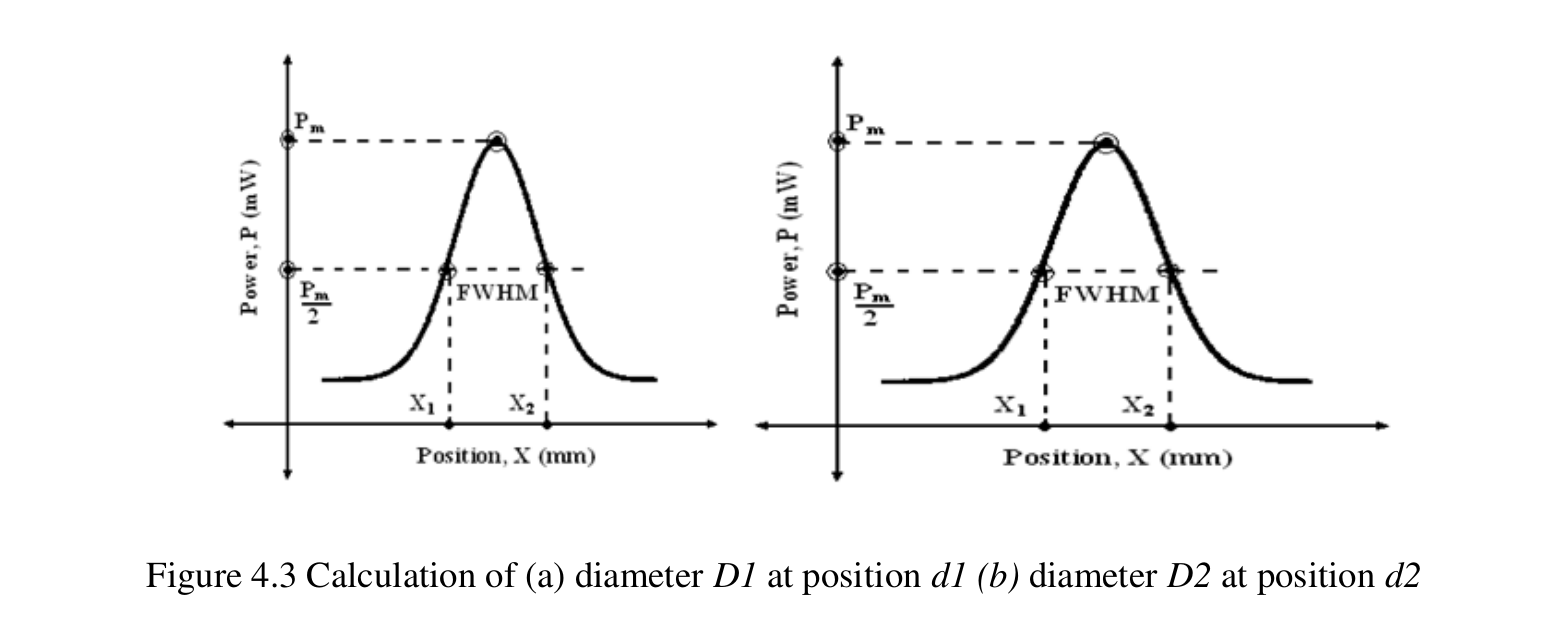
\includegraphics[scale=0.4]{2.png}
		\label{it}
	\end{figure}
	
	\section{Graphs}
\subsection{Plot between $\textit{Power} (mW)$ vs $\textit{Position} x(mm)$ at Distance d1 = 100 cm}
\begin{figure}[H]
	\centering
	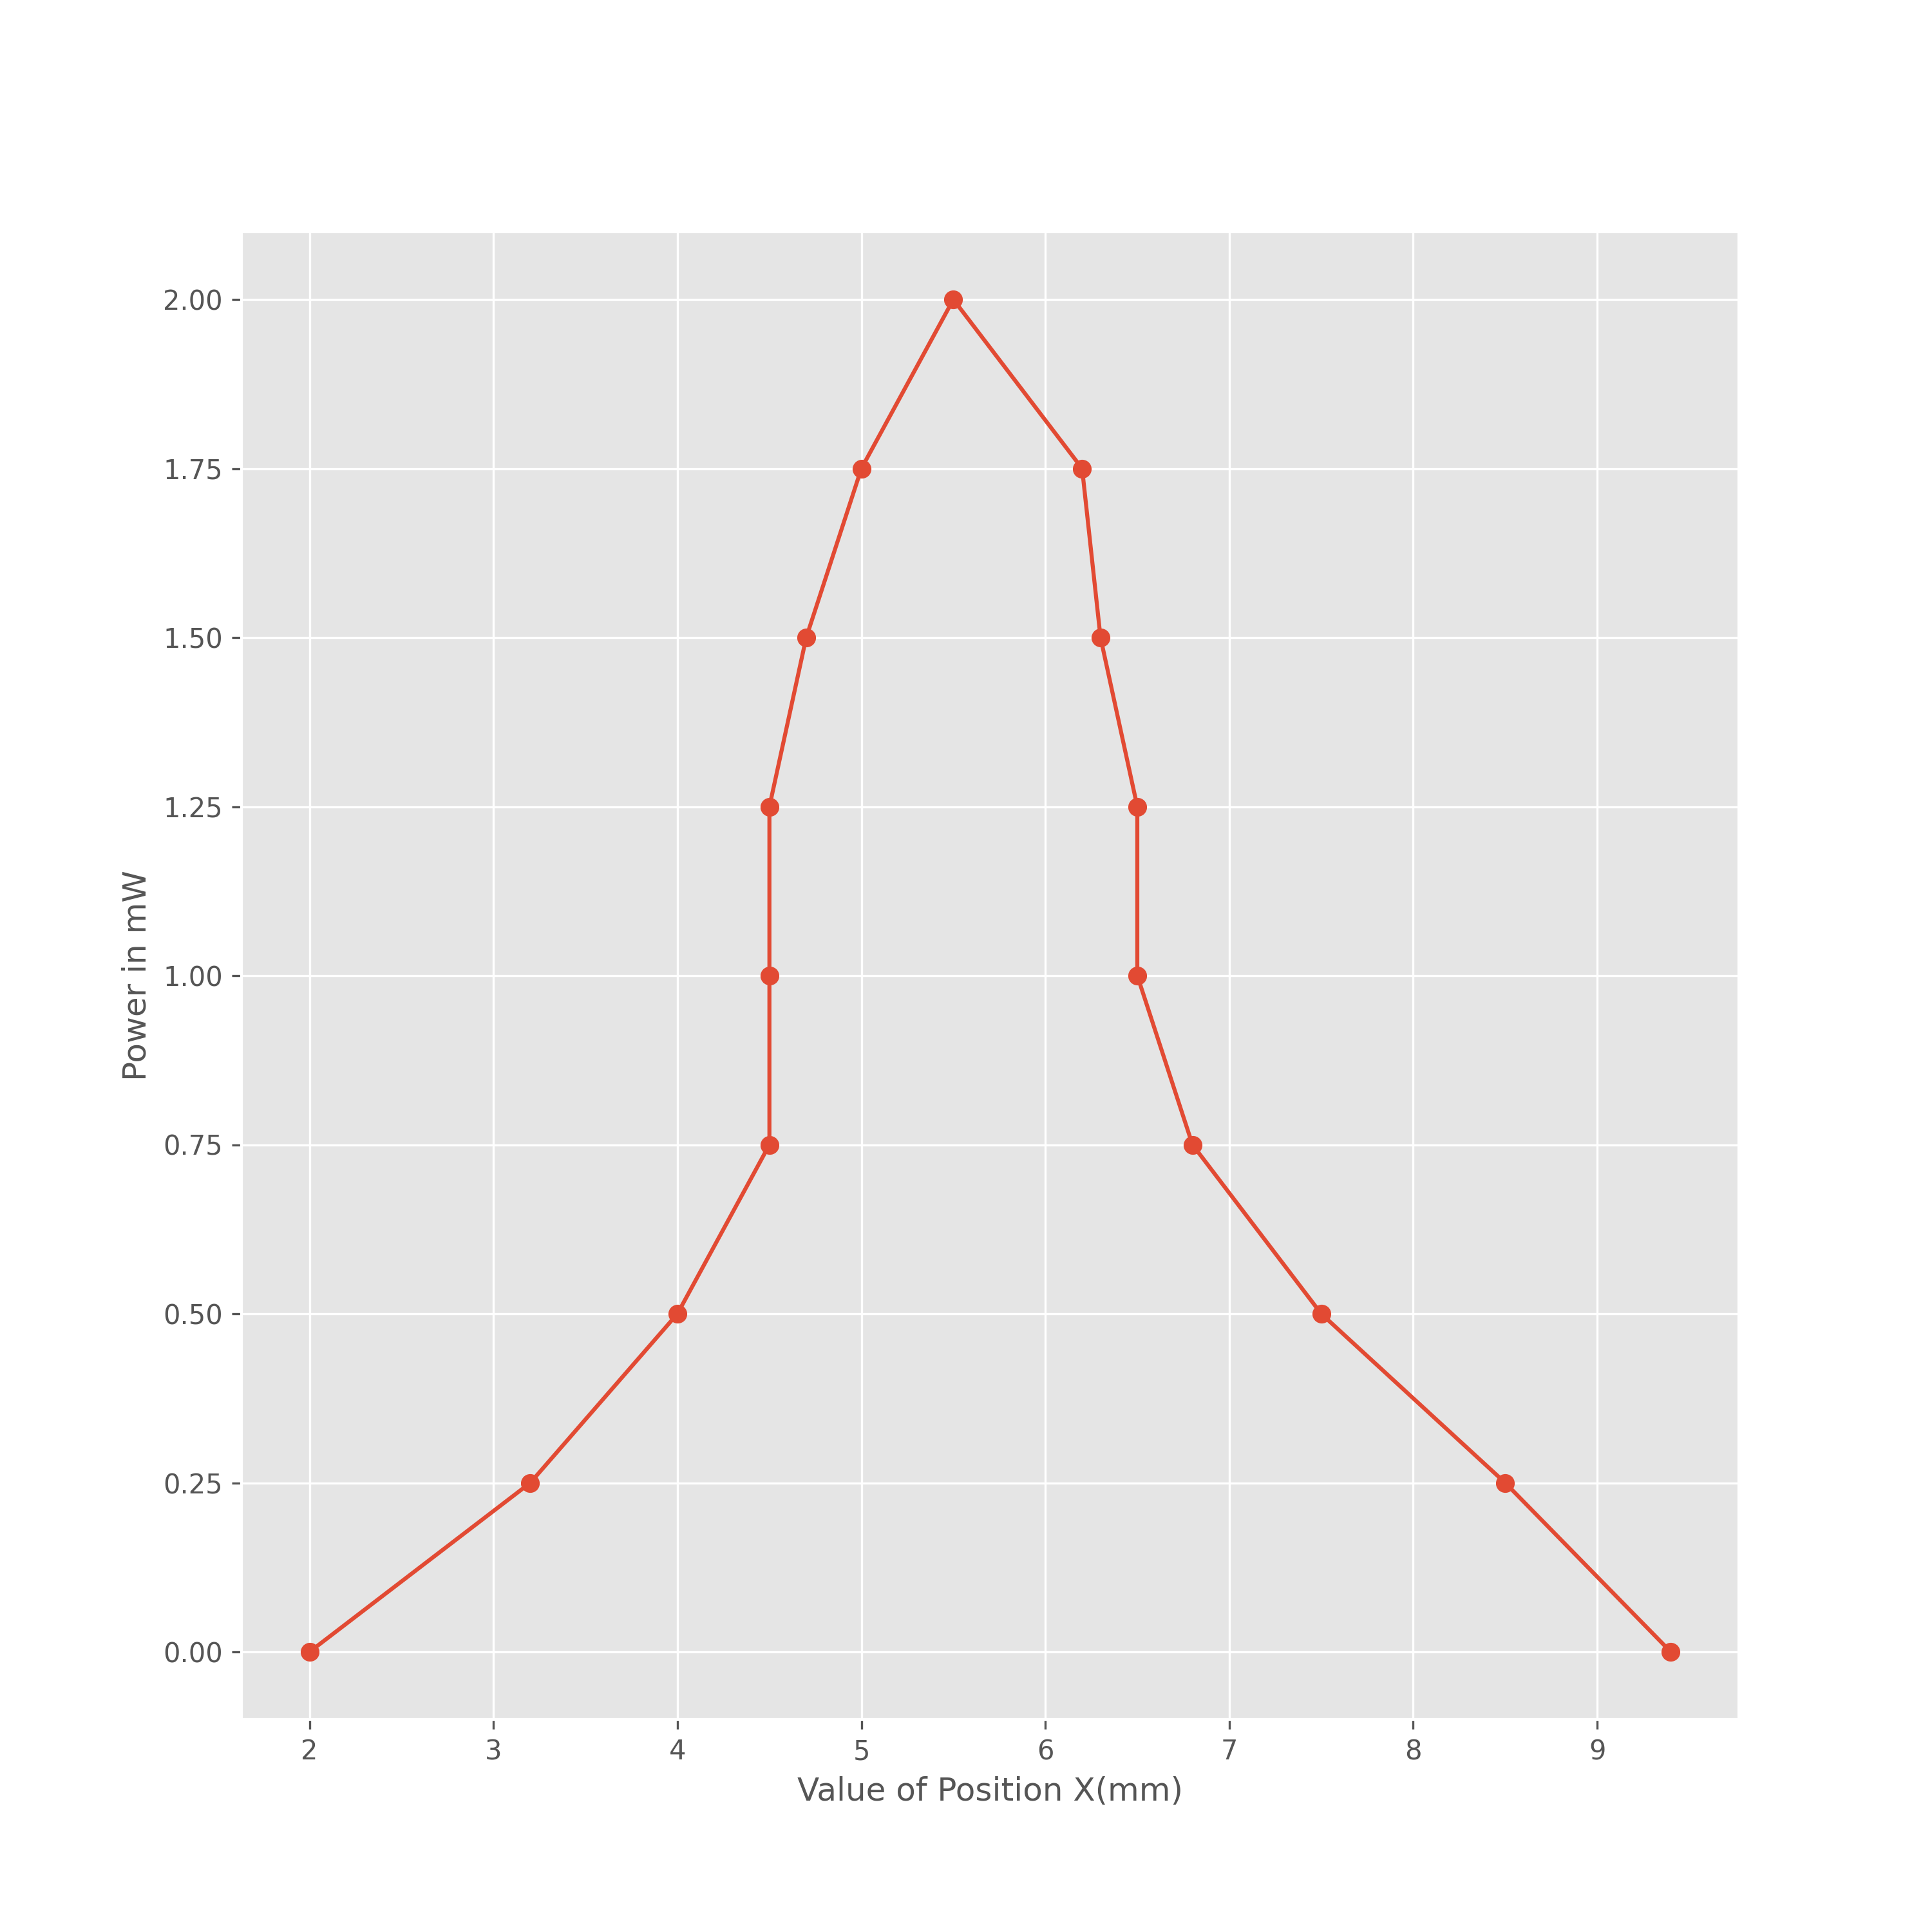
\includegraphics[scale=0.6]{fig.png}
	\label{it}
\end{figure}

\subsection{Plot between $\textit{Power} (mW)$ vs $\textit{Position} x(mm)$ at Distance d2 = 80 cm}
\begin{figure}[H]
	\centering
	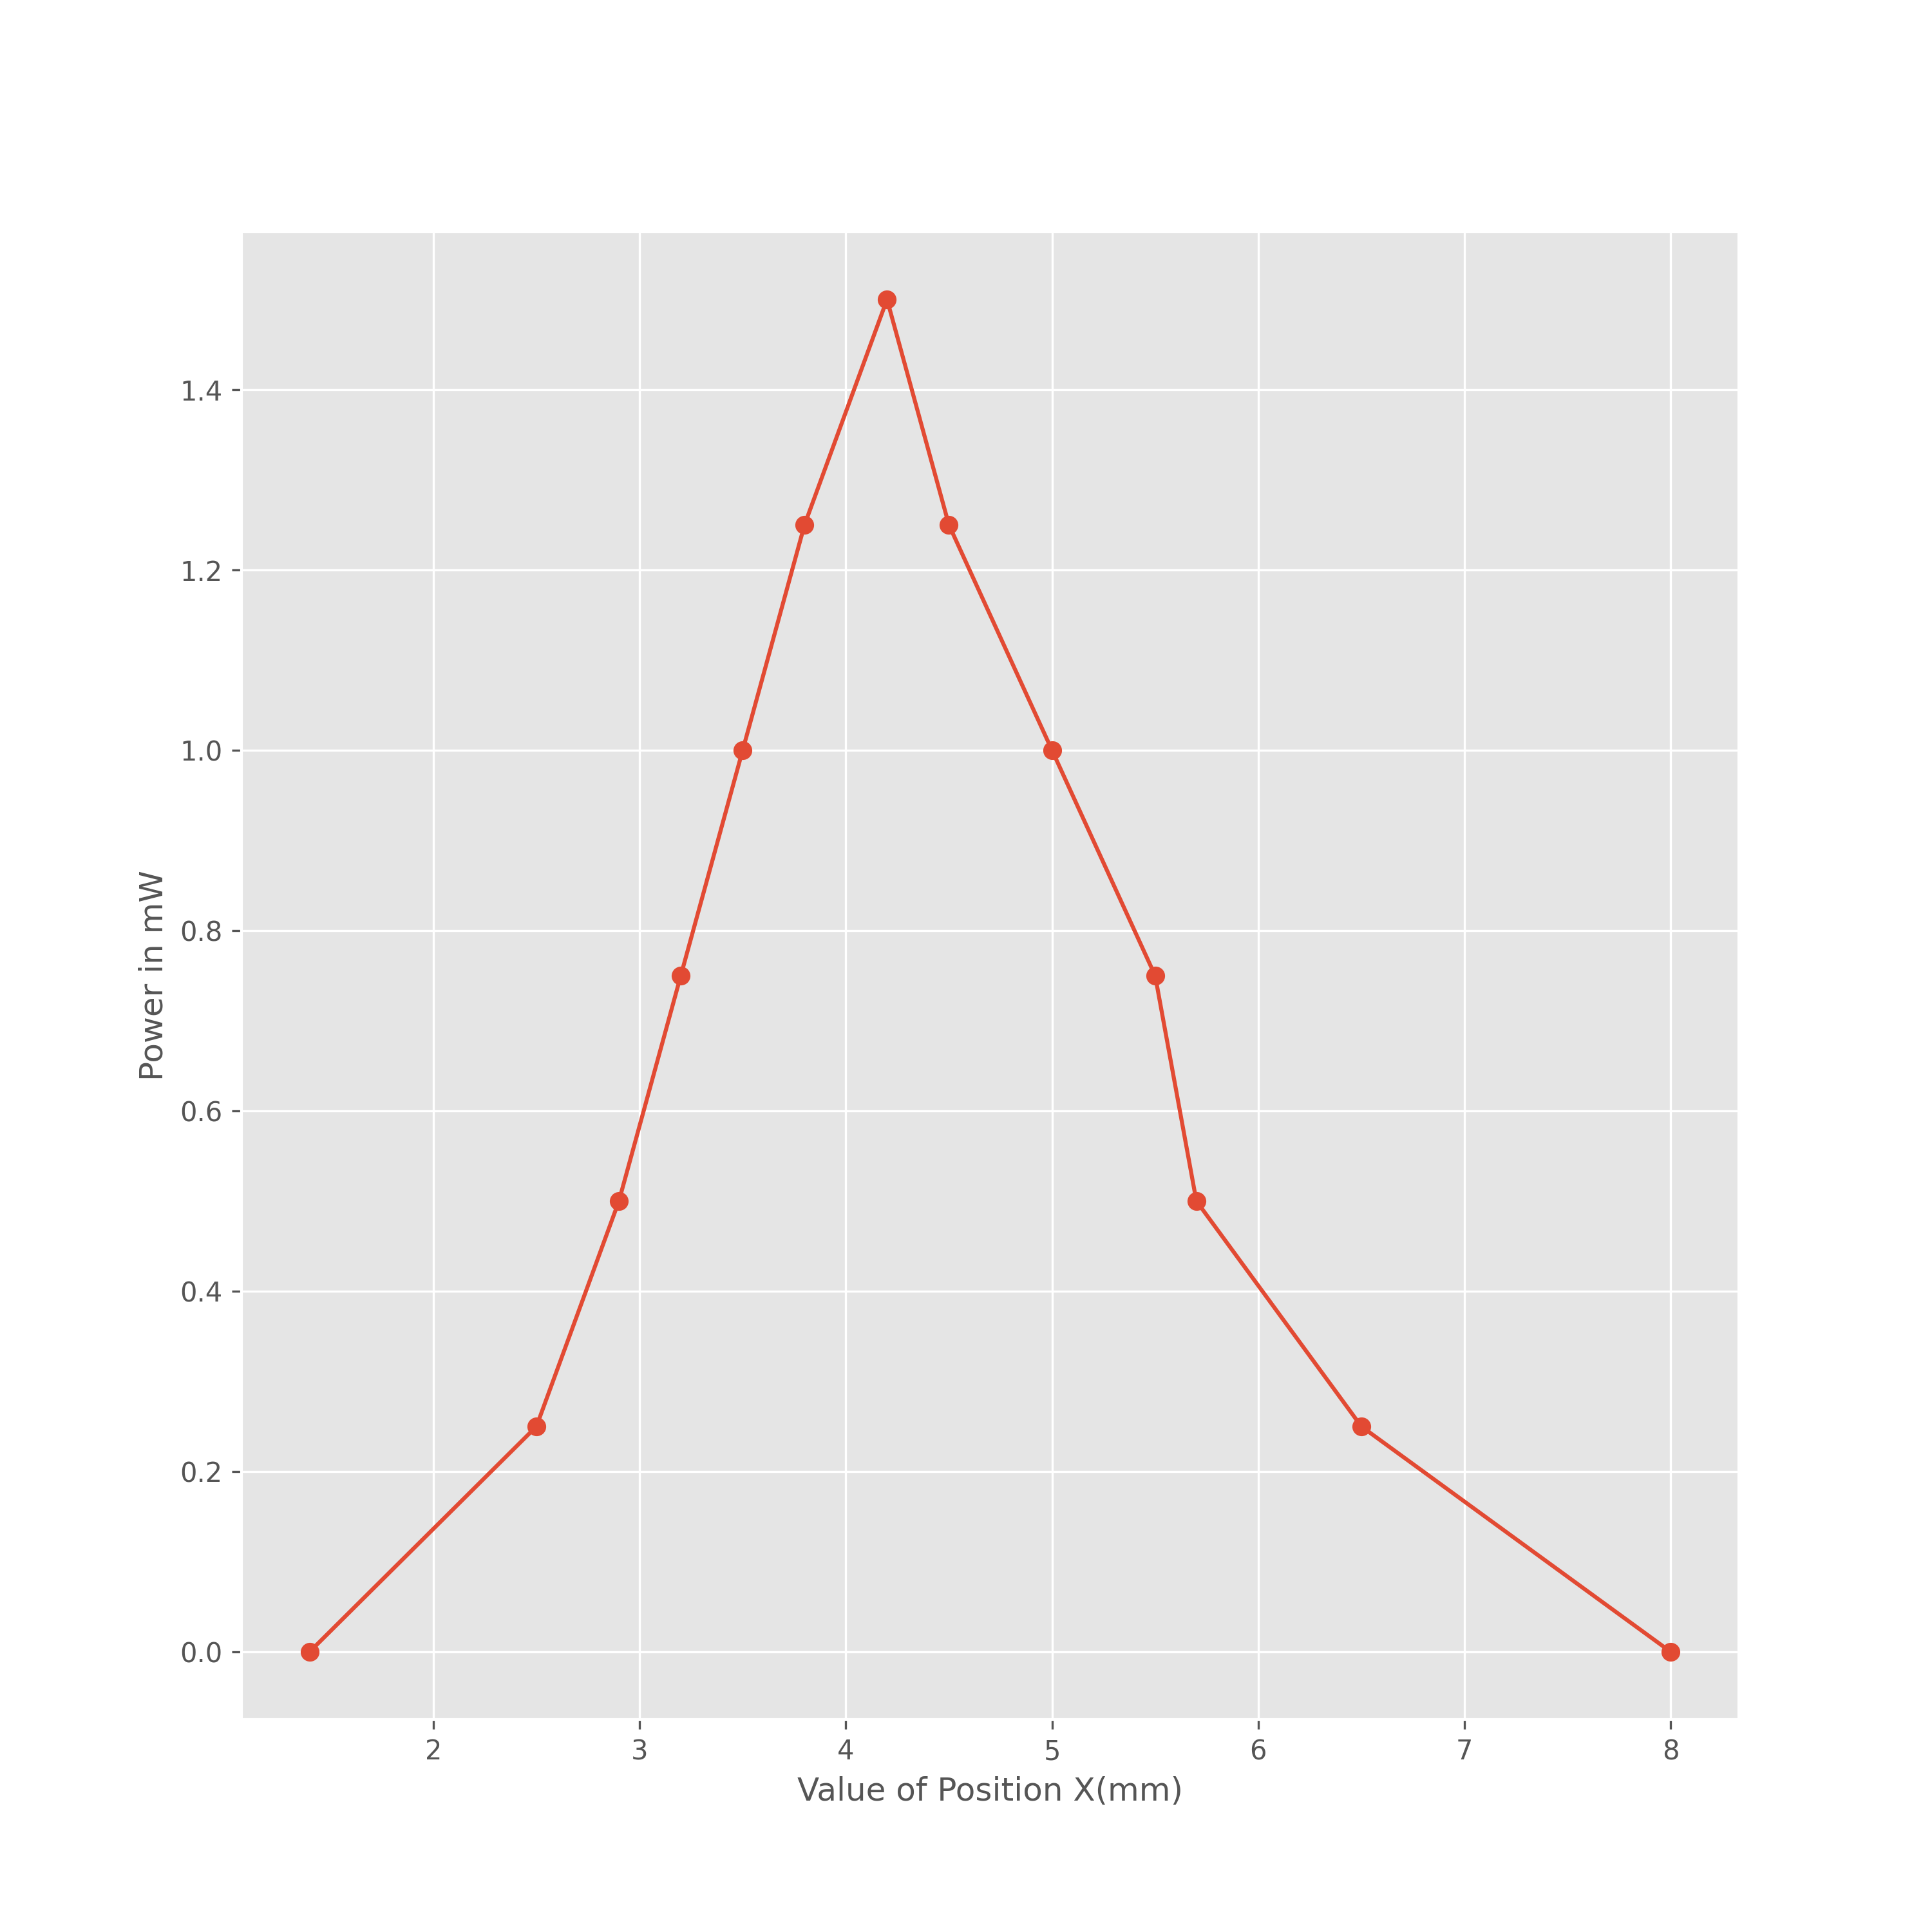
\includegraphics[scale=0.6]{fig2.png}
	\label{it}
\end{figure}

\section{My Understanding of the Experiment}
A Laser is an almost monochromatic unidirectional beam of light, that has been amplified by stimulated emission of Radiation. It has great significance in the medical and engineering world. 
One of the main reasons for this, is that it is a powerful beam of light that travels highly in the same direction and for a long distance. This is an experiment to verify that fact, and measure
the divergence of the laser beam after travelling a certain distance. That can be calculated by a laser beam analyser. 


\end{document}